\documentclass[12pt,a4paper]{article}
\usepackage{amsmath}
\usepackage{mathtext}
\usepackage{icomma}
\usepackage{amsfonts}
\usepackage{amssymb}
\usepackage[utf8]{inputenc}
\usepackage[T1,T2A]{fontenc}
\usepackage[english, russian]{babel}
\usepackage{graphicx}
\usepackage[left=2cm,right=2cm,top=2cm,bottom=2cm]{geometry}
\usepackage{calc}
\usepackage{wrapfig}
\usepackage{setspace}
\usepackage{indentfirst}
\usepackage{subfigure}
\usepackage[table,xcdraw]{xcolor}


\title{
Отчет о выполнении лабораторной работы 2.1.1 \\
Измерение удельной теплоемкости воздуха при постоянном давлении}

\author{Исламов Сардор, группа Б02-111}
\date{7 февраля 2022 г. }

\begin{document}
\maketitle

\subparagraph*{Аннотация.}
В работе изучена зависимость повышения температуры от мощности подводимого тепла и расхода при стационарном течении через трубу. Исключив тепловые потери, по результатам измерений определена теплоемкость воздуха при постоянном давлении.

\subsection*{Теоретические сведения}
Теплоемкость тела в некотором процессе определяется как отношение подводимого к телу тепла и изменения его температуры:
\begin{equation}
    C = \frac {\delta Q} {dT}
\end{equation}

Надежность измерения зависит от качества установки. Необходимо, чтобы количество тепла, затрачиваемого на нагрев тела, во много превосходило тепло, расходуемое на нагрев установки и потерю тепла в окружающую среду.

Рассмотрим газ, протекающий стационарно слево направо через трубу постоянного сечения, в которой установлен нагревательный элемент мощностью $N$ (рис. 1).
\begin{figure}[htp]
\centering
    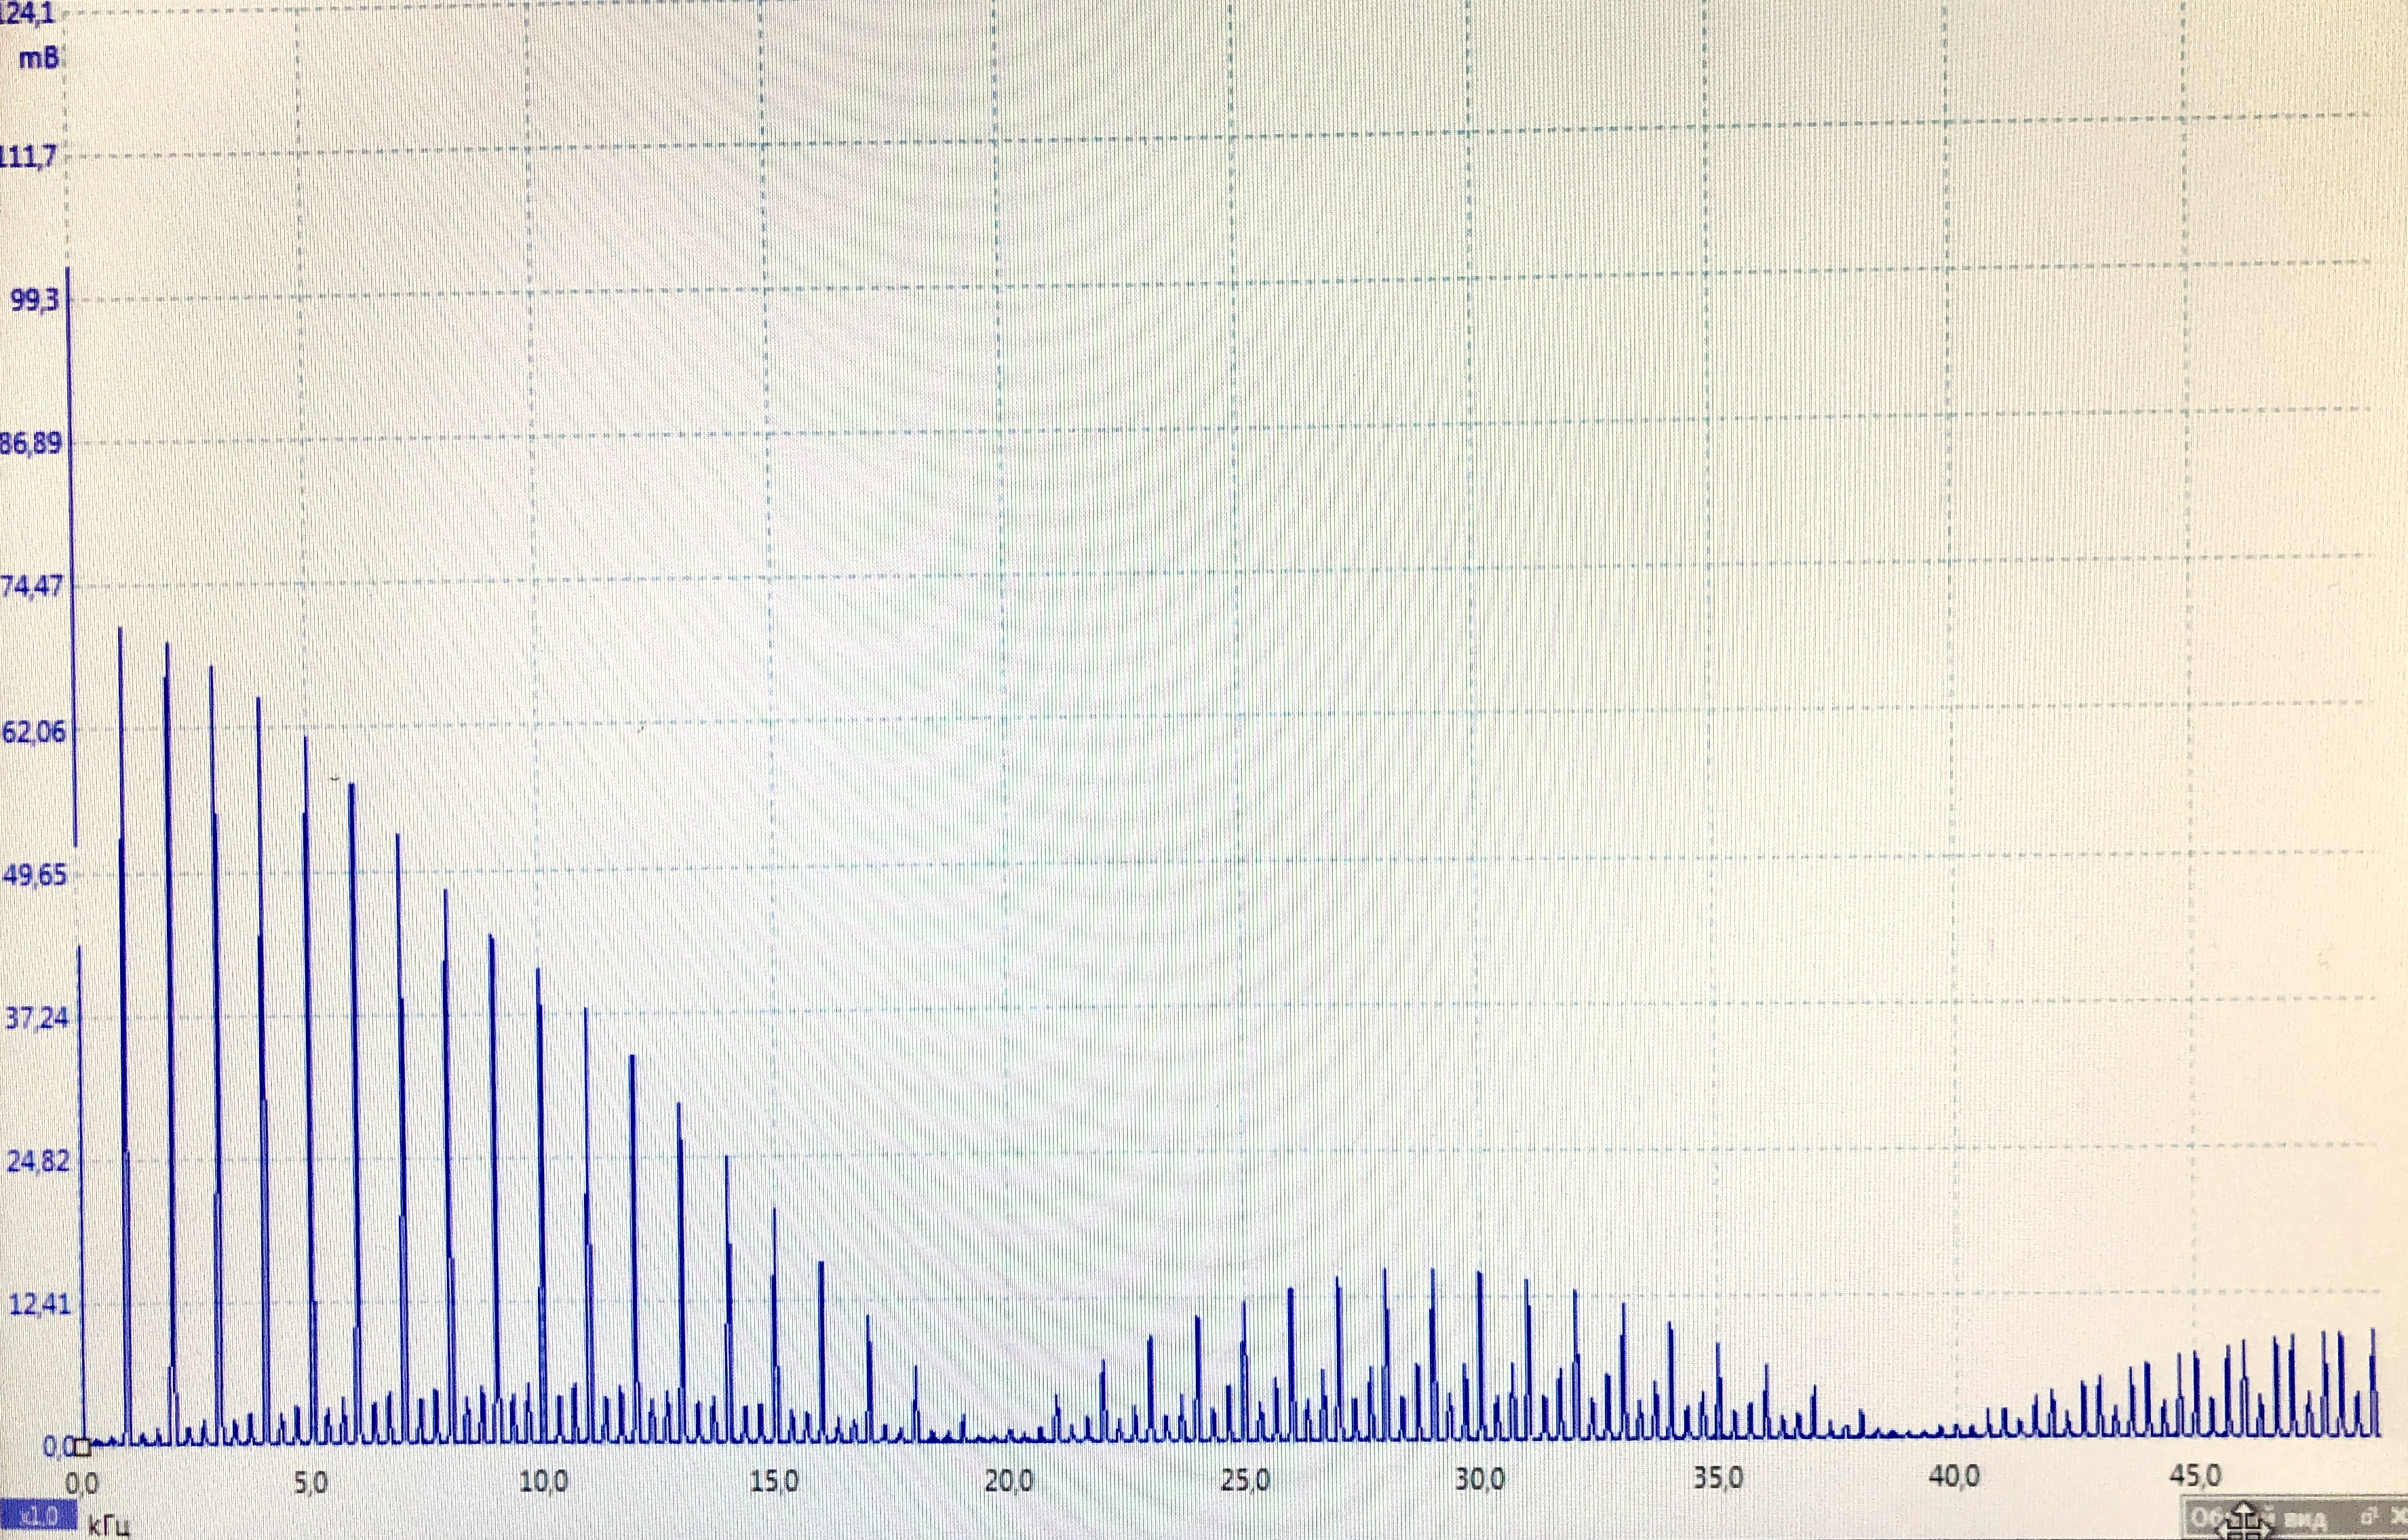
\includegraphics[width=0.5\linewidth]{1.png}
    \caption{Нагрев газа при течении по трубе}
    \label{fig:my_label}
\end{figure}

Пусть за некоторое время $dt$ через калориметр прошла малая порция газа массой $dm=q dt$, где $q$ [кг/с] — массовый расход газа в трубе. Если мощность тепловых потерь равна $N_{пот}$, то газ получил тепло $\delta Q=(N-N_{пот})dt$. С другой стороны $\delta Q = cdm \Delta T$, где $\Delta T = T_2-T_1$ - приращение температуры газа, и $c$ - удельная теплоемкость газа в этом процессе. При малых расходах газа и большом диаметре трубы перепад давления на ее концах мал, т.е. можно принять, что $P_1\approx P_2 \approx P_0$, где $P_0$ - атмосферное давление. Таким образом получаем выражение для удельной теплоемкости при постоянном давлении 
\begin{equation}
    c_p=\frac{N-N_{пот}}{q\Delta T}
\end{equation}

\subsection*{Экспериментальные методы}
\subparagraph*{В работе используются:}теплоизолированная стеклянная трубка; электронагреватель; источник питания постоянного тока; амперметр, вольтметр (цифровые мультиметры); термопара, подключенная к микровольтметру; компрессор; газовый счётчик; секундомер.

Схема установки изображена на рис. 2
\begin{figure}[h!]
    \centering
    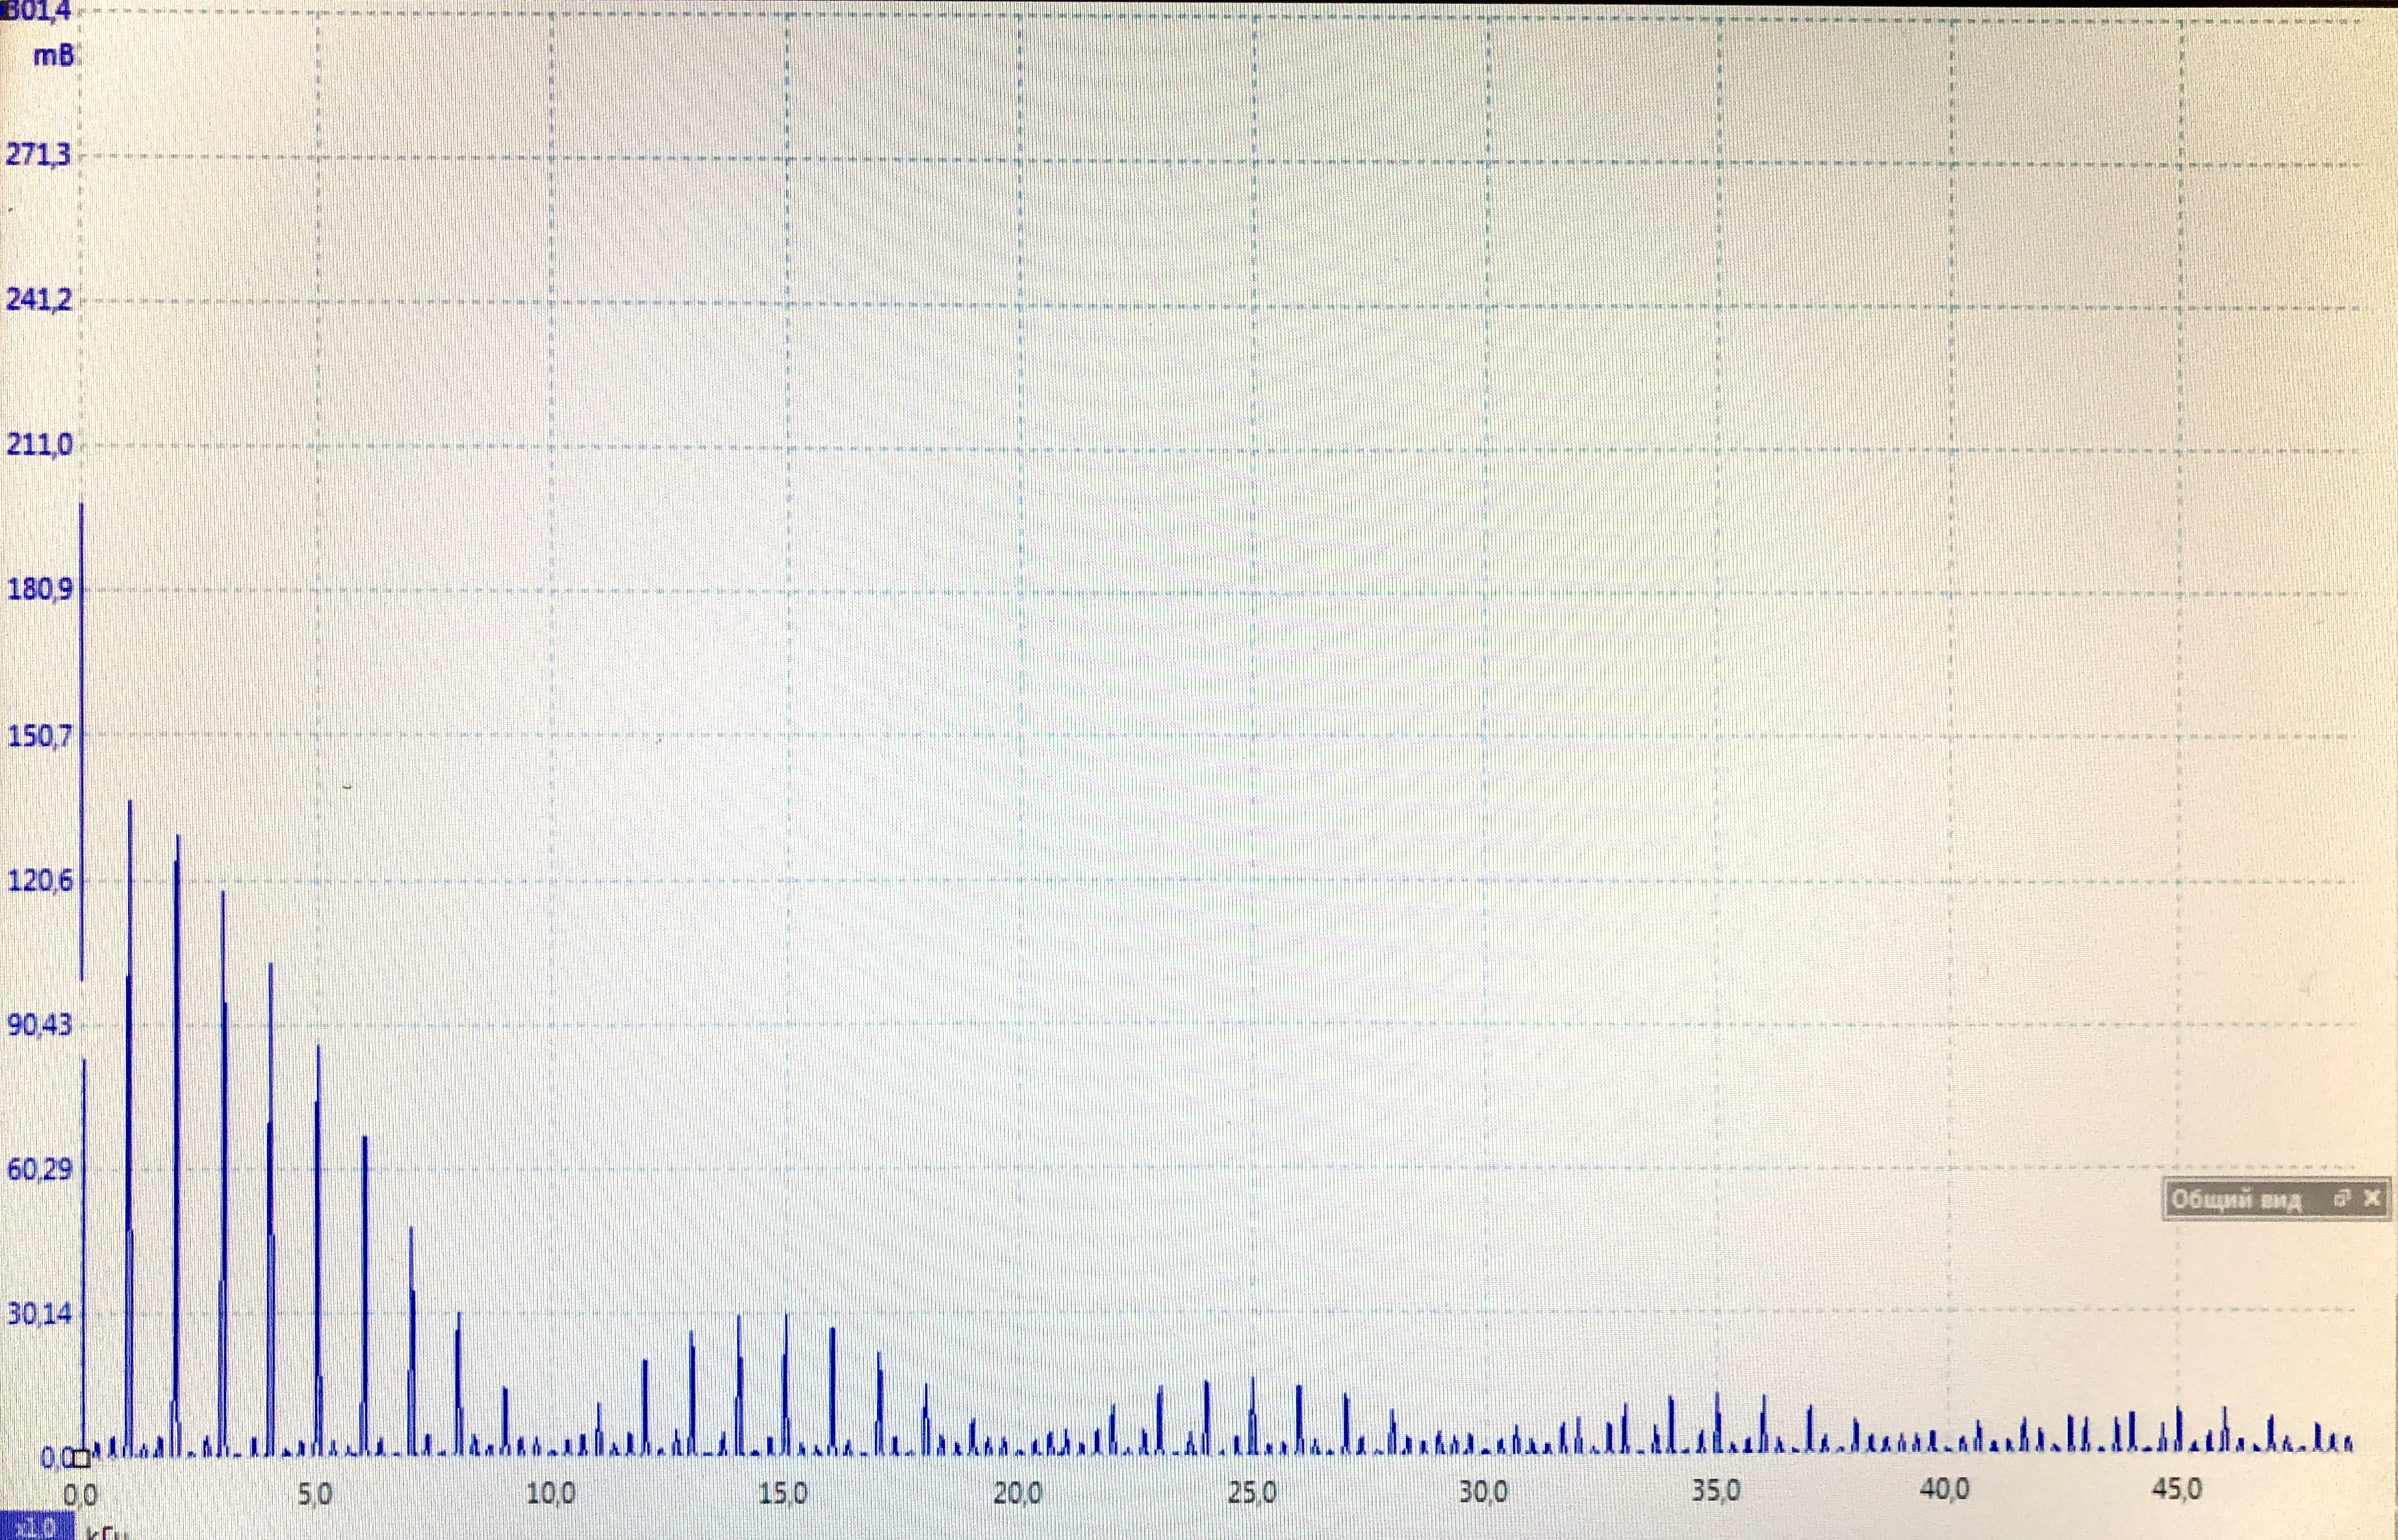
\includegraphics[width=0.7\linewidth]{2.png}
    \caption{Схема экспериментальной установки}
    \label{fig:my_label}
\end{figure}

Воздух, нагнетаемый компрессором, прокачивается через калориметр. Калориметр представляет собой стеклянную цилиндрическую трубку с двойными стенками, запаянными с торцов. На внутреннюю поверхность стенок трубки нанесено серебряное покрытие для минимизации потерь тепла засчет излучения. Воздух из пространства между стенками калориметра откачан до высокого вакуума $10^{-5} торр$ для минимизации потерб тепла, обусловленных теплопроводностью.

Нагреватель в виде намотанной на пенопласт нихромовой проволоки расположен внутри калориметра непосредственно в воздушном потоке. Нагрев проволоки производится от регулируемого источника постоянного тока (ИП).
Напряжение $U$ на нагревателе и ток $I$ через него регистрируются цифровыми мультиметрами. Таким образом, мощность нагрева равна
\begin{equation}
    N =UI
\end{equation}

Для измерения разности температур $\Delta T$ служит медно-константановая
термопара. Один спай термопары расположен в струе воздуха, входящего в калориметр, и находится при комнатной температуре, а второй — в струе выходящего нагретого воздуха. Константановая проволока термопары расположена внутри калориметра, а медные проводники подключены к цифровому вольтметру. Возникающая в термопаре ЭДС $\varepsilon$ пропорциональна разности температур $\Delta T$ спаев:
\begin{equation}
    \varepsilon =\beta \Delta T  
\end{equation}
где $\beta = 40.7 \frac{мкВ}{^\circ C}$ — чувствительность медно-константановой термопары в рабочем диапазоне температур (20–30 $^\circ C$ ). ЭДС регистрируется с помощью микровольтметра.

Объём воздуха, прошедшего через калориметр, измеряется газовым счётчиком ГС. Для регулировки расхода служит кран К. Время $\Delta t$ прохождения
некоторого объема $\Delta V$ воздуха измеряется секундомером. Объёмный расход равен $\frac{\Delta V}{\Delta t} $, массовый расход может быть найден как 
\begin{equation}
    q = \rho_{0} \frac{\Delta V}{\Delta t}
\end{equation} 
где $\rho_{0}$ — плотность воздуха при комнатной температуре, которая в свою очередь может быть получена из уравнения Менделеева–Клапейрона: $\rho_{0}= \frac{\mu P_{0} }{R T_{0}},$ где $P_{0}$ — атмосферное давление, $T_{0}$ — комнатная температура (в Кельвинах), $\mu = 29,0 {г/моль}$ — средняя молярная масса (сухого) воздуха.

Учитывая особенности устройства калориметра, следует ожидать, что мощность нагревателя расходуется не только на нагрев массы прокачиваемого воздуха, но и частично теряется за счет нагрева внутренних стенок термостата и рассеяния тепла через торцы термостата. Можно предположить, что при небольшом нагреве ($\Delta T \ll T_{0}$) мощность потерь тепла $N_{пот}$ прямо пропорциональна разности температур:
\begin{equation}
    N_{пот} = \alpha \Delta T
\end{equation}
где $\alpha$ — некоторая константа. При этом условии основное соотношение (2) принимает вид 
\begin{equation}
    N = (c_{p}q +\alpha)\Delta T 
\end{equation}
Следовательно, при фиксированном расходе воздуха ($q = const$ ) подводимая мощность и разность температур связаны прямой пропорциональностью($\Delta T(N)$ — линейная функция).

\subsection*{Методика измерений и обработка данных}
\begin{enumerate}
    \item Подготовим к работе газовый счетчик: проверим, заполнен ли он водой, установим счетчик по уровню.
    
    \item Начинать измерения следует при условии, что калориметр охлажден до комнатной температуры. Для охлаждения включим компрессор и открывая кран К, установим максимально возможный расход воздуха. Источник постоянного тока должен быть при этом выключен.
    
    \item Снимем показания давления, температуры и относительной влажности в комнате.
    \begin{table}[ht!]
    \begin{center}
    \begin{tabular}{|c|c|c|c|c|c|}
    \hline
    $P, кПа$ & $\sigma_P, кПа$ & $T, ^oC$ & $\sigma_T, ^oC$ & $\varphi$ & $\sigma_\varphi$\\ \hline
           98.325 &   0.001& 22  &   0.1&  48 &1 
            \\ \hline
    \end{tabular}
    \caption{Характерные параметры воздуха в помещении}
    \end{center}
    \end{table}
    
    \item С помощью газового счетчика и секундомера измерим максимальный расход воздуха $\Delta V / \Delta t$ в л/с. Максимальный расход $q_{max}$ расчитаем по формуле (5).
    \begin{equation*}
        \rho_0 = 1.163\ кг/м^3,\ 
        \sigma_\rho = \rho_0 \sqrt{\left(\frac {\sigma_p}{P_0} \right)^2 + \left(\frac {\sigma_T}{T_0} \right)^2}\approx 0.005 \ кг/м^3
    \end{equation*}
    \begin{table}[ht!]
    \begin{center}
    \begin{tabular}{|c|c|c|c|c|c|}
    \hline
    $\Delta V,  л$ & $\sigma_V, л$ & $\Delta t, c$ & $\sigma_t, c$ & $q_{max}, г/с$ & $\sigma_q, г/с$, \\ \hline
        15.0 &   0.1&  74.5 &   0.5&  0.235 &  0.002     
        \\ \hline
        15.0 &   0.1&  74.7&   0.5&  0.235 &        0.002          
        \\ \hline
        15.0&   0.1&  74.6 &  0.5 &  0.235 &             0.002     
        \\ \hline
    \end{tabular}
    \caption{Измерения для $q=0.235\ г/с$}
    \end{center}
    \end{table}
    \item Оценим величину тока нагревателя $I_0$, требуемого для нагрева воздуха на $\Delta T = 1^oC$. Для этого 
    \begin{enumerate}
        \item [5.1]Определим теоретическое значение удельной теплоемкости воздуха при постоянном давлении $c_p^{теор} \approx 10^3 Дж/кг\ К$, считая воздух смесью идеальных двухатомных газов;
        \item [5.2]Оценим минимальную мощность $N_0\ (N\ge c_p q \Delta T)$, необходимую для нагрева газа при максимальном расходе $q_{max}$ на $\Delta T = 1^oC$. $N_0=0.235\ Вт$;
        \item [5.3]Учитывая что сопровтивление проволоки нагревателя составляет приблизительно $R_н\approx 35\ Ом$ и в процессе опыта практически не меняется, определим искомое значение тока
        \begin{equation*}
            I_0 = \sqrt{\frac {N_0}{R_н}}\approx 81,94мА.
        \end{equation*}
    \end{enumerate}
    
    \item Проведем измерение зависимости разности температур от мощности нагрева $\Delta T(N)$ при максимальном расходе воздуха $q_1 = q_{max}$. 
    \begin{enumerate}
        \item[6.1] Чтобы начать нагрев, включим источник питания (ИП) нагревателя и установим на нем такое напряжение, чтобы ток через нить накаливания составлял $I_1 \sim (2 \div 2.5)I_0$. Запишем значения тока $I$ и напряжения $U$ в цепи. Расчитаем мощность нагрева $N$, а также сопротивление нити нагревателя $R_н$.
        \item[6.2] После включения нагрева (или после изменения его мощности) дождемся установления стационарного состояния системы.
        \item[6.3] По величине $\varepsilon$ определим значение $\Delta T$. Учитывая, что $\Delta T \sim N \sim I^2$, определим значения токов канала, необходимые для того, чтобы равномерно повышать температуру нагрева $\Delta T$ до требуемого значения. Проведем измерения согласно пп. 6.1-6.2, последовательно увеличивая ток нагрева до расчетных значений.
        
        \begin{table}[ht!]
        \begin{center}
        \begin{tabular}{|c|c|c|c|c|c|c|c|c|c|}
        \hline
        $I, мА$ & $\sigma_I, мА$ & $U, В$ & $\sigma_U, В$ & $N, мВт$ & $\sigma_N, мВт$ & $\varepsilon, \mu В$ & $\sigma_\varepsilon, \mu В$ & $\Delta T, K$ & $\sigma_T, K$ \\ \hline
                77.09&  0.01&  2.73& 0.01 &  210.38&  0.68& 29 &1  & 0.71 &    0.02          
                \\ \hline
                89.98&  0.01&3.18  &  0.01&  286.50&  0.93& 41 &1  &  1.01& 0.02
                \\ \hline
                118.56&  0.01&4.19  &  0.01&  497.0&  1.6&72  & 1 &  1.77&               0.02
                \\ \hline
                135.04&  0.01&4.77  &  0.02& 644.4 & 2.1 &95 & 1 &  2.33&             0.02  
                \\ \hline
                163.86&  0.02&5.79  & 0.02 &  948.6&  3.1&140  &1  & 3.44 &0.02
                \\ \hline
        \end{tabular}
        \caption{Измерения для $q=0.235\ г/с$}
        \end{center}
        \end{table}
    \end{enumerate}
    \item Проведем измерения для другого значения расхода воздуха. Соответствующие значения занесем в таблицы (4) и (5).
     \begin{table}[ht!]
    \begin{center}
    \begin{tabular}{|c|c|c|c|c|c|}
    \hline
    $\Delta V,  л$ & $\sigma_V, л$ & $\Delta t, с$ & $\sigma_t, с$ & $q_{max}, г/с$ & $\sigma_q, г/с$, \\ \hline
        15.0 &   0.1&  99.9&   0.5&   0.175&    0.002   
        \\ \hline
        15.0&   0.1&   100.2&   0.5&  0.174 &        0.002          
        \\ \hline
        15.0&  0.1 &   100.0&   0.5&   0.174&             0.002     
        \\ \hline
    \end{tabular}
    \caption{Измерения для $q=0.174\ г/с$}
    \end{center}
    \end{table}
    
    \begin{table}[ht!]
        \centering
        \begin{tabular}{|c|c|c|c|c|c|c|c|c|c|}
        \hline
        $I, мА$ & $\sigma_I, мА$ & $U, В$ & $\sigma_U, В$ & $N, Вт$ & $\sigma_N, Вт$ & $\varepsilon, \mu В$ & $\sigma_\varepsilon, \mu В$ & $\Delta T, K$ & $\sigma_T, K$ \\ \hline
                63.09&  0.01&  2.25& 0.01 &  141.74& 0.45 &23  &1  &0.57  &              0.02
                \\ \hline
                79.88&  0.01& 2.84 &  0.01&  226.62&  0.73&40  &1  & 0.98&0.02
                \\ \hline
                113.19& 0.01 &4.01  &  0.01& 453.7 &  1.5&85  & 1 & 2.09 &               0.02
                \\ \hline
                142.52&  0.01&5.03  &  0.02&717.0  &  2.3&144  &1  &  3.54&               0.02
                \\ \hline
                179.84&  0.02&  6.35&  0.02&  1141.1&  3.7&  225&1  &5.53  &0.02
                \\ \hline
        \end{tabular}
        \caption{Измерения для $q=0.174\ г/с$}
        % \end{center}
        \end{table}
        \begin{figure}
        \begin{flushright}
            \includegraphics[width = 0.2\linewidth]{sign.png}
            \label{fig:my_label}
        \end{flushright}
        \end{figure}
    \item Построим графики зависимости $\Delta T(N)$ для каждого значения расхода воздуха $q$. Видно, что точки хорошо ложатся на прямую, значит тепловые потери пропорциональны разности температур. Коэффициенты наклона прямых найдем по МНК.
    \begin{equation*}
        k_1 = (3.60\pm 0.02)\cdot 10^{-3}Вт/К,\ k_2 = (4.82\pm 0.06)\cdot 10^{-3}Вт/К.
    \end{equation*}
    
    \begin{figure}[ht!]
        \centering
        \includegraphics[width=0.7 \linewidth]{tn.png}
        \caption{Графики зависимости $\Delta T(N)$}
        \label{fig:my_label}
    \end{figure}
    
    \item Пользуясь формулой (7) и полученными значениями получаем
    \begin{equation*}
        c_p = \frac{\frac{N_1}{\Delta T_1}-\frac{N_2}{\Delta T_2}}{q_1-q_2} = \frac{\frac{1}{k_1}-\frac{1}{k_2}}{q_1-q_2} = 1152 \frac{Дж}{кг\ К}
    \end{equation*}
    \begin{equation*}
        \sigma_{c_p} = \sqrt{\left(\frac {\partial c_p}{\partial k_1} \sigma_{k_1}\right)^2+\left(\frac {\partial c_p}{\partial k_2} \sigma_{k_2}\right)^2+\left(\frac {\partial c_p}{\partial q_1} \sigma_{q_1}\right)^2+\left(\frac {\partial c_p}{\partial q_2} \sigma_{q_2}\right)^2} =
    \end{equation*}
    \begin{equation*}
        =\sqrt{\left(\frac {\sigma_{k_1}}{k_1^2(q_1-q_2)} \right)^2+ \left(\frac {\sigma_{k_2}}{k_2^2(q_1-q_2)} \right)^2+ \left(\frac {\sigma_{c_p q_1}}{q_1-q_2} \right)^2+ \left(\frac {\sigma_{c_p q_2}}{q_1-q_2} \right)^2} \approx 75 \frac{Дж}{кг\ К}
    \end{equation*}
    Теперь, пользуясь полученным значением $c_p$ и формулой (7), определим $\frac{N_{пот}}{N}$.
    \begin{equation*}
        N = c_p q \Delta T + N_{пот} \Rightarrow \frac{N_{пот}}{N} = 1-c_p q_1 k_1 \approx 0.025
    \end{equation*}
    \begin{equation*}
        \sigma_{N_{пот}/N} = N_{пот}/N\sqrt{\left( \frac{\sigma_{c_p}}{c_p}\right)^2+\left( \frac{\sigma_{q_1}}{q_1}\right)^2+\left( \frac{\sigma_{k_1}}{k_1}\right)^2} \approx 0.002
    \end{equation*}
\end{enumerate}

\subsection*{Вывод}
В ходе работы изучена зависимость повышения температуры от мощности подводимого тепла и расхода при стационарном течении через трубу. На основе полученных данных выяснено, что тепловые потери пропорциональны разнице температур. Исключив потери тепла, отношение которых к подводимой мощности составляет $\frac{N_{пот}}{N} = 0.025\pm0.002\ (\varepsilon = 8\%)$, определена удельная теплоемкость воздуха при постоянном давлении $c_p = (1152\pm75)\frac{Дж}{кг\ К}\ (\varepsilon = 7\%)$. Небольшое отличие полученного значениея от табличного $c_p = 1000\frac{Дж}{кг\ К}$ может быть связано с высокой влажностью воздуха в помещении, неучитывающейся при расчете плотности.
\end{document}
